\documentclass[12pt]{article}
\usepackage[user]{cqd}
\usepackage{graphicx} 
\usepackage{amsmath}
\usepackage{amsfonts}
\usepackage{hyperref}
\usepackage{latexsym}
\usepackage[brazil]{varioref}
\usepackage[english,brazil]{babel} 
\usepackage{float}
\usepackage{listings}
%\usepackage[dvips]{color}






 \newtheorem{teo}{Teorema}%[subsection]
 \newtheorem{cor}[teo]{Corolário}
 \newtheorem{lem}[teo]{Lema}
 \newtheorem{prop}[teo]{Proposição}
 \newtheorem{defn}[teo]{Definição}
% \newtheorem{nota}[teo]{Nota}
 \newtheorem{obs}[teo]{Observação}
% \newtheorem{exemplo}[teo]{Exemplo}
 %\newtheorem{proof}{Demonstração}
 \newcommand{\pr}{\hspace*{.6cm}}  %parágrafo´, usar apenas no início da seção ou subseção
 \newenvironment{proof}{\noindent{\it Demonstra\c{c}\~ao.} }{\hfill $\Box$ \newline}





\newcommand{\mP }{\mathbb{P}}
\newcommand{\me}{\mathbb{E}}
\newcommand{\mn}{\mathbb{N}}
\newcommand{\mr }{ \mathbb{R}}
\newcommand{\dive}{\textrm{div}_E }
\newcommand{\grade}{\textrm{grad}_E }
\newcommand{\grad}{\textrm{grad}}
\newcommand{\eop }{ \hfill $\blacksquare$ }
\newcommand{\I }{\textbf{\textrm{i}}}
\newcommand{\D }{\textbf{\textrm{d}}}
\newcommand{\s}{\textbf{\textrm{S}}}
\newcommand{\F}{\mathcal{F}}
\newcommand{\M}{\mathcal{M}}
\newcommand{\N}{\mathcal{N}}
\newcommand{\sS}{\mathcal{S}}


%% amsmath já carregado
%%\RequirePackage[utf8]{inputenc} já carregado
%\RequirePackage{etoolbox} já carregado
%\RequirePackage{color} já carregado
%\RequirePackage{calc} já carregado
%\RequirePackage[english,brazil]{babel} já carregado
%\RequirePackage{graphicx} já carregado
%\RequirePackage{geometry} já carregado

%% ambientes 'newtheorem' já disponíveis: 
%%  - teorema, corolario, lema, proposicao,
%%  - definicao, nota, observacao, exemplo, 
%%  - exercicio
%%
%%%%%%%%%%%%%%%%%%%%%%%%%%%%%%%%%%%%
%% preencha as informações abaixo %%

\titulo{ Estudo analítico e computacional de uma equação diferencial estocástica associada a um modelo de crescimento populacional}
\tituloingles{Analytical and computational study of a stochastic differential equation associated to a population growth model}

\autor{Hitalo Cesar Alves}{Instituto de Computação}{UNICAMP}{hitalo.c.a@gmail.com }{Alves, H. S.}
\autor{Diego Sebastian Ledesma}{IMECC}{UNICAMP}{ledesma@unicamp.br}{Ledesma, D. S.}
 


\resumo{Neste trabalho estudamos  uma equação diferencial estocástica associada a modelos de crescimento populacional. Em particular achamos sua solução analítica e a uma medida invariante para a equação. Logo simulamos por métodos computacionais a solução e comparamos com o obtido analíticamente. }

\palavraschave{Equações diferenciais estocásticas. Simulação de processos estocásticos. Modelo de crescimento populacional.}


\abstract{In this work, we study a stochastic differential equation associated with population growth models. In particular, we find its analytical solution and an invariant measure for the equation. Then we simulate the solution by computational methods and we compare it with the one obtained analytically.
}

\keywords{Stochastic differential equations. Simulation of stochastic processes. Population growth model.}


\begin{document}
\section{Introdução}

As equações diferenciais estocásticas são uma ferramenta muito importante na modelagem matemática de processos que ocorrem na natureza, fundamentalmente, porque permite a introdução de tudo aquilo que não é possível quantificar (por sua quantidade de variáveis ou sua pouca relevância para o processo) por meio de um ruído nos coeficientes do modelo.

O objetivo deste trabalho é dar uma ideia sobre como trabalhar com equações diferenciais estocásticas estudando a modo de exemplo, por métodos analíticos e computacionais,  um caso em particular. Por isto, neste trabalho, consideramos uma equação diferencial estocástica não linear associada a modelos de crescimento populacional e que é dada por 
\begin{eqnarray*}
dx_t=rx_t(k-\alpha x_t)~dt+\beta x_tdB_t \quad x_0=N
\end{eqnarray*}
para $N,~r,~k,$ e $\alpha\in[0,\infty]$ e tais que $2rk>\beta^2$.
Esta é uma pequena variação de um modelo proposto por Polansky(1979) e nos permite, por meio de  variações do parámetro $\alpha$, estudar um conjunto de equações que incluem o modelo já mencionado de Polansky ($\alpha=1$) e o bem conhecido modelo estândar de crescimento populacional com ruido (OKSENDAL, 1997) para ($\alpha=0$). 

O artigo será dividido em três partes. Na primeira parte faremos uma breve revisão da teoria básica de equações diferenciais estocásticas. Logo depois introduzimos a equação diferencial estocástica a ser trabalhada e provamos o resultado principal do trabalho que diz sobre a existência de solução e da medida invariante para esta. Finalmente, na terceira parte, fazemos uma breve revisão da teoria de simulações para equaçoes diferenciais estocásticas pelo modelo de Euler e fazemos a simulação da solução utilizando a linguagem Python. Logo, comparamos os resultados modelados com os obtidos analíticamente.  

Este trabalho faz parte do estudo de Iniciação Científica do primeiro autor. 


\section{Breve revisão de cálculo estocástico}
Nesta seção pretendemos dar brevemente a fundamentação teórica do trabalho. Expomos brevemente os resultados principais e indicamos as referências onde podem ser achados para uma revisão mais aprofundada do tópico.  


Fixamos, ao longo do trabalho, um espaço de probabilidade filtrado $(\Omega,\{\mathcal{F}_t\}_{t\in I},\mP)$ para $I\subset \mr$.
\begin{defn}
Se $(\Omega,\mathcal{F},\mP)$ é um espaço de probabilidade, uma variável aleatória real $X$ é uma função $\mathcal{F}_t$ mensurável $X:\Omega\rightarrow \mr$. Dada uma variável aleatória $X:\Omega\rightarrow \mr$ definimos a sua lei $F_X:\mr\rightarrow [0,1]$ como sendo a medida de probabilidade sobre $\mr$ tal que 
\[
F_X(U)=\mP[X^{-1}(U)]
\]
\end{defn}

Seja $X:\Omega\rightarrow \mr$ uma variável aleatória  e $f:\mr\rightarrow \mr$, definimos o seu valor esperado  (ou esperança) de $f(X)$ como o número $\me[f(X)]$ obtido da seguinte forma
\[
\me[f(X)]=\int_\Omega f(X)~d\mP=\int_\mr f(x)~dF_X(x).
\]


\begin{defn}  
Um processo estocástico real é um conjunto de variáveis aleatórias $\{X_t:\Omega\rightarrow \mr\}$ indexadas por um  parámetro $t$ tomando valores num conjunto ordenado (usualmente $\mathbb{N}$ ou $\mr$)
\end{defn}
Neste trabalho vamos nos concentrar no caso em que o parámetro $t$ toma valores em um intervalo $I\subset \mr$. O processo estocástico mais importante para os nossos estudos é o Movimento Browniano. Este é o processo $\{B_t\}_{t \geq 0}$ com as seguintes propriedades:  
\begin{itemize}
\item $B_0 = 0$
\item a função $t \rightarrow B_t$ é contínua em $t$,
\item o processo $\{B_t\}_{t \geq 0}$ tem incrementos estacionários e independentes, os incrementos $B_{t+s}-B_s$ tem por lei a distribuição normal com média $0$ e variância $t$. Ou seja: $B_{t+s}-B_s \sim N(0,t)$.
\end{itemize}
\'E possível mostrar, utilizando o teorema de continuidade de Kolmogorov (ver, por exemplo, o capítulo 2 do livro de OKSENDAL, B.), que o movimento browniano pode ser construído de forma tal que os seu caminhos, isto é, as funções 
\[t\in[0,\infty)\rightarrow X_t(\omega)\in  \mr,\] sejam contínuos . Então, cabe a pergunta se é possível integrar com respeito a $B_t$. Nesse sentido é definida a integral de Itô, como sendo 
\[
\int_0^tf(s,B_s)~dB_s=\lim_{n\rightarrow\infty}\sum_{t_i\in \tau_n,~t_i\leq t}f(s_i,B_{t_i})(B_{t_{i+1}}-B_{t_i})\quad(\textrm{limite em}~L^2(\Omega,\mP))
\]onde  $f:\mr\times\mr\rightarrow \mr$ é uma função $C^\infty$, $B_t$ é o movimento browniano
e $\{\tau_n\}$ uma sequ\^encia de parti\c{c}\~oes de $[0,t]$  tais que 
\[
 |\tau_n|=\sup_n|t_{i+1}-t_i|\rightarrow 0\hspace{1cm}\textrm{se}~n\rightarrow\infty.
\]
É possível ver que 
\begin{itemize}
\item a integral de Itô é independente da sequência de partições,
\item  o processo \[
A_t=\int_0^tf(s,B_s)~dB_s
\]
é um processo estocástico $F_t$ mensurável para cada $t$  com 
\[
\me\left[A_t\right]=0,
\]
para todo $t$ (SONDERMAN, 2006).
\end{itemize}

A integral de Itô não obedece a fórmula de mudança de variáveis. No seu lugar temos a bem conhecida \textbf{fórmula de Itô} que é o equivalente estocástico ao teorema fundamental do cálculo. Apresentamos aqui uma versão simplificada desta: 

\begin{teo}
Seja $f:\mr\times \mr^n\rightarrow \mr$ uma função $C^\infty$ e $\{B_t\}$ o movimento browniano iniciando em $B_0=x$ então 
\[
f(t,B_t)=f(0,x)+\int_0^t\partial_xf(s,B_s)~dB_s+\int_0^t\left[(\partial_tf)(s,B_s)+\frac{1}{2}\partial_x^2f(s,B_s)\right]~ds,\] ou na forma diferencial 
\[
df(t,B_t)= \partial_xf(t,B_t)~dB_t+ \left[(\partial_tf)(t,B_t)+\frac{1}{2}\partial_x^2f(t,B_t)\right]~dt,\]

\end{teo}
Para uma prova do resultado consultar o capítulo 3 do livro de OKSENDAL, B.
\begin{exemplo}
Em particular, se $f:\mr\times \mr^2\rightarrow \mr$ dada por 
\[
f(t,x)=g(t)h(t,x)
\]
onde $g(t)$ é um processo que admite derivada com respeito a $t$ e $h$ uma função $C^\infty$, temos que a fórmula de Itô garante
\[
f(t,B_t)=f(0,0)+\int_0^t\left(\dot{g}(s)+g(s)\partial_th(s,B_s)+\frac{1}{2}g(s)\partial_x^2h(s,B_s)\right)~ds+\int_0^tg(s)\partial_xh(s,B_s)~dB_s.
\]
ou na forma diferencial 
\[
df(t,B_t)=h(t,b_t)dg(t)+g(t)\left(\partial_th(t,B_t)+\frac{1}{2}\partial_x^2h(t,B_t)\right)~dt+g(t)\partial_xh(t,B_t)~dB_t
\]
\end{exemplo}

Uma vez conhecida a integral de Itô, definimos a \textbf{Equa\c{c}\~ao diferencial estoc\'astica no sentido It\^o} (EDE) a valores reais como sendo uma equação da forma 
\begin{eqnarray}\label{EDE}
 dx_t=X_0(t,x_t)~dt+ X_1 (t,x_t)~dB_t, \quad x_0=x,
\end{eqnarray}
onde $X_i:\mr\times \mr\rightarrow \mr$ são funções $C^\infty$.
Esta equação, embora escrita na forma diferencial, deve ser entendida na forma integral. Isso é o conteúdo da seguinte definição.
\begin{defn}
Seja $(s,x)\in[0,T]\times\mr^n$. Um processo estoc\'astico cont\'inuo $x_t$, para $t\in[s,T]$, a valores em $\mr $ \'e dito um solu\c{c}\~ao (forte) da equação diferencial estocástica (\ref{EDE}), com condi\c{c}\~ao inicial $x_s=x$ se, e somente se, satisfaz
\[
 x_t=x+\int_s^tX_0(r,x_r)~dr+ \int_s^tX_1(r,x_r)~dB_r .
\] 
\end{defn}



Em geral, garantir a existência e unicidade de soluções de equações diferenciais estocásticas não é fácil. Há resultados que garantem que se os coeficientes da equação são localmente Lifschitz é possível garantir a existência da solução (KUNITA, 1997). No entanto, achar uma forma explícita da solução pode ser uma tarefa muito difícil. 

Se $x_t$ é solução da equação \ref{EDE} então podemos provar, como consequência da fórmula de Itô, que para toda função $f\in C^2(\mr)$ temos  
\[
f(x_t)=f(x_0)+\int_0^t\left(X_0(r,x_r)\partial_xf(x_r)+\frac{1}{2}X_1(r,x_r)^2\partial_x^2f(x_r)\right)~dr+\int_0^tX_1(r,x_r)\partial_xf(x_r)~dB_r,
\]
ou, na forma diferencial,
\[
df(x_t)=\left(X_0(t,x_t)\partial_xf(x_t)+\frac{1}{2}X_1(t,x_t)^2\partial_x^2f(x_t)\right)~dt+X_1(t,x_t)\partial_xf(x_t)~dB_t.
\]
Para mais detalhes, consultar o capítulos 3 e 4 de OKSENDAL, B. 


Dada a equação diferecial estocástica \ref{EDE} como acima, assuma que existe uma aplicação \[\phi:[0,\infty)\times \mr\times \Omega\rightarrow \mr,\] contínua nas primeiras duas variáveis, e tal que para cada $x$ dá a solução \[x_t(\omega)=\phi(t,x,\omega)\] da equação com $x_0=x$. Tal aplicação é comumente chamada de fluxo solução.  Uma medida de probabilidade \[\mu=\rho(x)~dx\] é dita invariante  para a equação \ref{EDE} se 
\[
\me\left[ \int_{\mathbb{R}}f(\phi(t,x,\omega))\rho(x)~dx\right]=\int_{\mathbb{R}}f(x)\rho(x)~dx
\]
para toda $f\in C^\infty(\mathbb{R})$ e $t\in[0,\infty)$.

Vamos a interpretar qual o significado da medida invariante. Para isto, considere que para a equação \ref{EDE}  existe um ponto $y_0$ tal que 
\[
X_0(t,y_0)=0,\quad X_1(t,y_0)=0.
\]
Neste caso, o processo \[x_t=\phi(t,y_0,\omega)=y_0\] é solução natural da equação para $x_0=y_0$. Estes pontos são chamados de pontos de equilibrio para a equação. Em particular temos que medida dada pela delta de dirac $\delta_{y_0}(x)$ é uma medida invariante para a equação pois 
\begin{eqnarray*}
\me\left[\int_{\mathbb{R}}f(\phi(t,x,\omega)\delta_{y_0}(x)~dx\right]&=&\me\left[f(\phi(t,y_0,\omega)\right]\\
&=&f(y_0)\\
&=&\int_{\mathbb{R}}f(x)\delta_{y_0}(x)~dx.
\end{eqnarray*}
Assim, de forma geral, as medidas invariantes são generalizações dos pontos de equilibrio da equação estocástica. 

Podemos caracterizar as medidas invariantes utilizando um operador diferencial de segunda ordem 
\[
LV(x)= X_0(t,x)\partial_xV(x)+\frac{1}{2}X_1(t,x)^2\partial_x^2V(x).
\]
para toda função $V$ diferenciável. Este é o conteúdo do seguinte resultado.
\begin{lema} Uma
medida de probabilidade  $\mu(x)=\rho(x)~dx$ é invariante para a equação \ref{EDE} se 
\begin{eqnarray}\label{eqmedidainvariante}
\int_{\mathbb{R}}Lf(x)\rho(x)~dx=0,
\end{eqnarray} 
para toda $f$ de classe $C^\infty$ e limitada. 
\end{lema}

\begin{proof} Seja $f$ de classe $C^\infty$ e limitada e $\phi(t,x,~)$ o fluxo solução da equação \ref{EDE}. Observamos que $f\circ \phi(t,x,~)$ é $C^\infty$ e limitada. 

Consideramos a identidade
\[
\mathbb{E}[Lf(\phi(t,x,~)]=L\mathbb{E}[f(\phi(t,x,~)]
\]
cuja prova pode ser encontrada em Oksendal(1997, p. 134,135). 



Da fórmula de Itô temos 
\[
f(\phi(t,x,~)=f(x)+\int_0^tf(\phi(s,x,~))~dB_s+\int_0^tLf(\phi(s,x,~)~ds
\]
Multiplicando por $\rho(x)$ e integrando obtemos 
\begin{eqnarray*}
\int_{ \mathbb{R}}f(\phi(t,x,~)\rho(x)~dx&=&\int_{ \mathbb{R}}f(x)\rho(x)+\int_0^t\left(\int_{ \mathbb{R}}f(\phi(s,x,~))\rho(x)~dx\right)~dB_s\\
&&+\int_0^t\int_{ \mathbb{R}}(Lf(\phi(s,x,~))\rho(x))~dx~ds
\end{eqnarray*}
Tomando esperança aos dois lados da identidade e utilizando que a medida $\mu(x)=\rho(x)~dx$ é de probabilidade, vemos que ela será invariante se, e só se,  temos
\[
\int_0^t\int_{ \mathbb{R}}L\mathbb{E}\left[f(\phi_s(x,~))\right]\rho(x)~dx~ds=\int_0^t\int_{ \mathbb{R}}\mathbb{E}\left[Lf(\phi_s(x,~))\right]\rho(x)~dx~ds=0.
\]
Portanto a medida será invariante se, e somente se, 
\[
\int_{\mathbb{R}}Lf(x)\rho(x)~dx=0,
\]
para toda $f$ de classe $C^\infty$ e limitada. 

\end{proof}



Mais ainda, podemos ver que para a medida invariante $\mu$ vale o seguinte resultado, de acordo com o Teorema 4.3 de Khasminskii(2011) ou o teorema 5.9 de Gard(1988)
\begin{teo}\label{khansminskii} Assuma que existe um conjunto $U$ aberto e limitado de $\mathbb{R}$ com fronteira regular $B$ tal que: 
\begin{itemize}
\item [a-]  $X_1(t,x)|_U>0$
\item [b-] Se $x\in U^C$ o tempo de saída $\tau$ de $U^C$ é finito. Isto é, se 
\[
\tau^x=\inf\{t,~\phi(t,x,\omega)\in U \},
\]
então $ \mathbb{E}\left[\tau^x\right]<\infty.$
Mais ainda, $\sup_{x\in K}\mathbb{E}[\tau^x]<\infty$ para todo compacto $K\subset \mathbb{R}$.
\item [c-] Se $\mu$ é a medida invariante associada à \ref{EDE} então $\mu(B)=0$ .
\end{itemize}
Então  
\[
\lim_{t\rightarrow \infty}\mathbb{P}[x_t\in A]=\int_A~d\mu.
\]
\end{teo} 

Este resultado é muito interessante pois, basicamente, diz que se a equação satisfaz as hipóteses podemos estudar o que aconetece (em probabilidade) com $x_t$ quando $t\to\infty$. 

Passamos a estudar agora condições sobre a equação \ref{EDE} que garantem que  esta satisfaz as hipóteses do teorema. Para isso, fazemos uma redução na equação \ref{EDE}, em particular pedimos que os termos que dirigem a equação sejam independentes do tempo, isto é, 
\[
X_0(t,x)=X_0(x)\quad \textrm{e}\quad X_1(t,x)=X_1(x)>0.
\] Desta forma, a equação satisfaz $a-$. Para mostrar $b-$ , considere agora a função $v$ de classe $C^2$ tal que 
\begin{eqnarray*}
Lv(x)=X_0(x)\partial_xv(x)+\frac{1}{2}X_1(x)^2\partial_x^2v(x)=-1.
\end{eqnarray*}
A escolha do valor $-1$ aqui é por conveniência, podendo ser escolhido um valor $k<0$.
Podemos ver que 
\begin{eqnarray*}
v(x)&=&-\exp\left(-\int^x_{y_0} \frac{2X_0(y)}{X_1(y)^2}~dy\right)\int^x_{y_0} \frac{1}{X_1(z)^2}\exp\left(\int^z_{y_0}  \frac{2X_0(y)}{X_1(y)^2}~dy\right)~dz\\
&=& \int^{y_0}_x \frac{1}{X_1(z)^2}\exp\left(-\int_z^x  \frac{2X_0(y)}{X_1(y)^2}~dy\right)~dz
\end{eqnarray*}
para algum $y_0\in \mr$, satisfaz a equação. Aplicamos agora a formula de Itô a $v(x_t)$ para obter 
\begin{eqnarray*}
v(x_T)&=&v(x_0)+\int_0^T\left(X_0(x)\partial_xv(x)+\frac{1}{2}X_1(x)^2\partial_x^2v(x)\right)~dt+\int_0^TX_1(x_t)\partial_xv(x)~dB_t\\
&=&v(x_0)-\int_0^T1~dt+\int_0^TX_1(x_t)\partial_xv(x)~dB_t.
\end{eqnarray*}
Então, se $\tau$ é a variável aleatória definida acima, vemos que 
\[
\mathbb{E}[v(x_{\tau})]=v(x_0)-\mathbb{E}[\tau].
\]
Portanto, se $v$ é uma função diferenciável e não negativa em $U^C$, vemos que 
\[\mathbb{E}[\tau]\leq v(x_0)<\infty\] e, consequêntemente, satisfaz as condições $a$ e $b$ do teorema (conforme teorema 3.11  de Khasminskii(2011)). Isto será exemplificado na próxima seção para um caso particular.  


\section{Modelo estocástico de crescimento populacional}

Nesta seção vamos aplicar os conceitos e resultados introduzidos na seção anterior para uma equação diferencial estocástica associada um modelo populacional . 

Consideramos a equação diferencial estocástica não linear dada por 
\begin{eqnarray}\label{crecimento}
dx_t=rx_t(k-\alpha x_t)~dt+\beta x_tdB_t, \quad x_0=N,
\end{eqnarray}
para $N,~r,~k,$ e $\alpha\in[0,\infty]$ e tais que $2rk>\beta^2$.

Esta equação é bem conhecida na literatura quando reduzida aos seguintes dois casos
\begin{itemize}
\item O caso em que $\alpha=0$ a equação se reduz à equação que modela o crecimento populacional estândar em que $rk$ é a taxa de crescimento e $\beta\in\mr$ é a medida do tamanho do ruído do ambiente.

\item O caso em que $\alpha=1$ a equação descreve o crescimento populacional em ambientes super-lotados. Nesse caso a constante $k>0$ é a capacidade do ambiente, $r>0$ é a medida da qualidade do ambiente  e $\beta\in\mr$ é a medida do tamanho do ruído do ambiente. 

% ver gard pag 171

\end{itemize}
Comparando a equação \ref{EDE} com a equação \ref{crecimento} temos 
\[
X_0(t,x)=rx(k-\alpha x)\quad \textrm{e}\quad X_1(t,x)=\beta x.
\]
Em particular, o operador $L$ é definido por 
\[
Lv(x)=rx(k-\alpha x)\partial_xv(x)+\frac{1}{2}\beta^2 x^2\partial_x^2v(x),
\]
para toda função $\nu$ de classe $C^\infty$.
No caso em que $\alpha=0$ a solução do problema $Lv=-1$ é
\[
v(x)=\frac{-2}{2rk-\beta^2} \ln(x),
\]
que é uma função que não é positiva definida portanto nada podemos garantir quanto à aplicação do teorema \ref{khansminskii}. No entanto, para $\alpha>0$ temos que a função 
\begin{eqnarray*}
v(x)&=& \frac{1}{\beta^2}x^{\left(\frac{2rk}{\beta^2}\right)}e^{-\left(\frac{2r\alpha}{\beta^2}x\right)}\int_x^\infty z^{\left(\frac{2rk}{\beta^2}\right)}e^{-\left(\frac{2r\alpha}{\beta^2}z\right)}~dz.
\end{eqnarray*}
é positiva e satisfaz $Lv=-1$ em $(0,\infty)$.
 
 
 Agora podemos provar o resultado principal do trabalho.

\begin{teo} \label{teoprincipal}
A equação diferencial estocástica  \ref{crecimento}
tem por solução 
\[
x_t=\frac{e^{\left(rk-\frac{1}{2}\beta^2\right)t+\beta B_t}}{\frac{1}{N}+r\alpha\int_0^te^{\left(rk-\frac{1}{2}\beta^2\right)s+\beta B_s}~ds}.
\]
Mas ainda, se $\alpha>0$, a equação admite uma medida invariante da forma $\mu=\rho(x)~dx$ para 
\[
\rho(x)=
\frac{1}{\Gamma\left(\frac{2rk}{\beta^2}-1\right)}
\left(\frac{2r\alpha}{\beta^2}\right)^{\left(\frac{2rk}{\beta^2}-1\right)}\exp\left(-\frac{2r\alpha}{\beta^2}x\right)
x^{\left(\frac{2rk}{\beta^2}-2\right)},
\]
donde $\Gamma$ é a função gamma que generaliza a função fatorial.  

\end{teo}
\begin{proof}
Propomos como solução um processo
\[
x_t=f(t)e^{\left(rk-\frac{1}{2}\beta^2\right)t+\beta B_t}
\]
Para $f(t)$ um processo que admita derivada com respeito a $t$ e tal que $f(0)=N$. Então,  calculamos 
\begin{eqnarray*}
dx_t&=&df(t)~e^{\left(rk-\frac{1}{2}\beta^2\right)t+\beta B_t}+f(t)(rk~dt+\beta~dB_t)e^{\left(rk-\frac{1}{2}\beta^2\right)t+\beta B_t}\\
&=&df(t)~e^{\left(rk-\frac{1}{2}\beta^2\right)t+\beta B_t}+rkx_t~dt+\beta x_t~dB_t.
\end{eqnarray*}
Comparando com a equação original, temos que $f(t)$ deve satisfazer 
\[
df(t)~=r\alpha f(t)^2e^{\left(rk-\frac{1}{2}\beta^2\right)t+\beta B_t}~dt.
\]
Portanto, 
\[
\frac{1}{f(t)}=\frac{1}{N}+r\alpha\int_0^te^{\left(rk-\frac{1}{2}\beta^2\right)s+\beta B_s}~ds.
\]
Juntando as partes temos então que a solução é
\[
x_t=\frac{e^{\left(rk-\frac{1}{2}\beta^2\right)t+\beta B_t}}{\frac{1}{N}+r\alpha\int_0^te^{\left(rk-\frac{1}{2}\beta^2\right)s+\beta B_s}~ds}.
\]
O fluxo solução é dado pelo mapa 
\[
\phi(t,x,\omega)=\left(\frac{e^{\left(rk-\frac{1}{2}\beta^2\right)t+\beta B_t}}{\frac{1}{x}+r\alpha\int_0^te^{\left(rk-\frac{1}{2}\beta^2\right)s+\beta B_s}~ds}\right)(\omega)
\]

 Observamos que a solução assume valores em $(0,\infty)$ então, é de esperar que a a medida invariante tenha soporte neste conjunto. Para achá-la, observamos que 
\[
Lf(x)=rx(k-\alpha x)\partial_xf(x)+\frac{1}{2}\beta^2 x^2\partial_x^2f(x).
\]
Então, se $\mu=\rho(x)~dx$ é invariante, temos que 
\[
\int_\mr\left(rx(k-\alpha x)\partial_xf(x)+\frac{1}{2}\beta^2 x^2f\partial_x^2f(x)\right)\rho(x)~dx=0
\]para toda função $f$ de classe $C^\infty$ e limitada. Assumindo que $\rho(x)$ é $C^2$, pelo fato de $\rho(x)$ ser a densidade de uma medida de propabilidade, temos que 
 \[
 \lim_{x\rightarrow \pm\infty}\rho(x)=0.
 \] 
 Agora, utiliando integração por partes e a limitação de $f$ vemos que 
 \begin{eqnarray*}
 \int_\mr\left(rx(k-\alpha x)\partial_xf(x)+\frac{1}{2}\beta^2 x^2f(x)\right)\rho(x)~dx&=& \int_\mr\partial_xf(x)\left(rx(k-\alpha x) \rho(x)\right)~dx\\
 &&+\int_\mr\left(\frac{1}{2}\beta^2 x^2\rho(x)\right) \partial_x^2 f(x)~dx\\
 &=&\int_\mr\partial_xf(x)\left(rx(k-\alpha x) \rho(x)\right)~dx\\
 &&+\int_\mr \partial_x^2 f(x)\left(\frac{1}{2}\beta^2 x^2\rho(x)\right)~dx\\
  &=&-\int_\mr f(x)\partial_x\left(rx(k-\alpha x) \rho(x)\right)~dx\\
 &&+\int_\mr f(x)\partial_x^2\left(\frac{1}{2}\beta^2 x^2\rho(x)\right)  ~dx
 \end{eqnarray*}
De onde obtemos que  
 \[
 \int_\mr\left(rx(k-\alpha x)\partial_xf(x)+\frac{1}{2}\beta^2 x^2f(x)\right)\rho(x)~dx=0\]
é equivalente a
 \[
\int_\mr\left(\partial_x\left(rx(k-\alpha x)\rho(x)\right)-\frac{1}{2}\beta^2 \partial_x^2(x^2\rho(x))\right)f(x)~dx=0
\]
para toda $f$ de classe $C^\infty$ e limitada.
 
 
 Portanto $\rho(x)$ resolve a equação 
\[ \partial_x\left(rx(k-\alpha x)\rho(x)\right)-\frac{1}{2}\beta^2 \partial_x^2(x^2\rho(x))=0.\]
Para resolvé-la, denotamos por 
\[
b(x)=rx(k-\alpha x),\quad \eta(x)=\frac{\beta^2}{2}x^2,
\]
então a equação pode ser simplificada a 
\[
\partial_x\left(b(x)\rho(x)-\partial_x(\eta(x)\rho(x))\right)=0
\]
Então 
\[
b(x)\rho(x)-\partial_x(\eta(x)\rho(x))=A
\]
para $A$ constante. Em particular para $A=0$, podemos escrever 
\[
\partial_x\left(\ln\left(\eta(x)\rho(x)\right)\right)=\frac{b(x)}{\eta(x)}
\]
De onde tiramos que, se $\alpha>0$, temos 
\[
\rho(x)=\frac{K}{\eta(x)}\exp\left(\int\frac{b(x)}{\eta(x)}dx\right)
\]
Substituindo pelos dados conhecidos, temos que 
\[
\rho(x)=K\exp\left(-\frac{2r\alpha}{\beta^2}x\right)
x^{\left(\frac{2rk}{\beta^2}-2\right)}
\]
para $K$ uma constante de renormalização. A forma de $\rho$ é similar com a da distribuição Gamma
\[h(x,a,b)=\frac{b^ax^{a-1}e^{-bx}}{\Gamma(a)} \] Portanto 
\[
\rho(x)=h(x,a,b)
\]
para 
\[
a=\frac{2rk}{\beta^2}-1,\quad b=\frac{2r\alpha}{\beta^2}\quad \textrm{e}\quad 
K=\frac{b^a}{\Gamma(a)}.
\]

\end{proof}

Uma vez que conhecemos a medida invariante podemos calcular, utilizando o teorema \ref{khansminskii}, qual a probabilidade de que um processo assuma valores em um determinado conjunto  $A$, quando o tempo é suficientemente grande, simplesmente calculando
\[
\lim_{t\rightarrow \infty}\mP[x_t\in A]=\int_A\rho(x)~dx.
\]
Observamos que isto só será possível se $\alpha>0$ pois o caso $\alpha=0$ não satisfaz o item $b-$ do teorema \ref{khansminskii}.
Para $\alpha>0$ temos que o máximo de $\rho(x)$ é atingido para 
\[
x_1=\frac{rk-\beta^2}{r\alpha}
\]
Então, calculando a integral da distribuição Gamma com os coeficientes como acima, podemos achar, para todo $\epsilon>0$, um intervalo da forma $A=(x_1-a,x_1+b)$ para $a,~b>0$ tais que
\[
\lim_{t\rightarrow \infty}\mP[x_t\in A]=1-\epsilon.
\]
Mais ainda, do que sabemos da distribuição gamma, podemos afirmar, qualitativamete, que o valor esperado de $x_\infty$ e a variancia $\sigma$ são 
\[
\me[x_\infty]=\frac{2rk-\beta^2}{2r\alpha},\quad\textrm{e}\quad\sigma(x_\infty)=\frac{\beta^2(2rk-\beta^2)}{(2r\alpha)^2}.
\]
Temos provado assim o seguinte resultado.
\begin{cor} Nas hipóteses do teorema \ref{teoprincipal} e com $\alpha>0$ temos  que para todo $\epsilon>0$ existem reais positivos $a,~b$ tais que se $A=(x_1-a,x_1+b)$ para 
\[
 x_1=\frac{rk-\beta^2}{r\alpha}
\]
então,
\[
\lim_{t\rightarrow \infty}\mP[x_t\in A]=1-\epsilon.
\]
\end{cor}
 

 

\section{Comparação analítica-computacional}

Nessa terceira parte estudamos a simulação da equação diferencial estocástica:

\[
dx_t=rx_t(k-\alpha x_t)dt+\beta x_tdB_t, \quad x_0=N,
\]
para $N,~r,~k,$ e $\alpha\in[0,\infty)$ e tais que $2rk>\beta^2$.\\

Começamos fazendo a simulação do movimento browniano. Observamos que esta deve ter as propriedades apresentadas na secção 2, isto é,  deve ser uma função $\{B_t: \Omega\rightarrow \mr\}$ tal que \begin{itemize}
\item $B_0=0$ 
\item se $t_0 = 0 < t_1 < t_2<...<t_l$, então o incremento $B_{t_i} - B_{t_{i-1}}$ é independente com $B_{t_i} - B_{t_{i-1}} \sim N(0,t_i-t_{i-1})$. Ou seja, $B_{t_i} - B_{t_{i-1}}$ não depende de $B_{t_{i-1}}$.
\end{itemize}
Para  simular uma função desse tipo, podemos gerar uma sequência de  variáveis aleatórias independentes $(S_j)_j$ e tais que $S_j \sim N(0,1)$. Mas como estamos trabalhando com o computador, queremos definir e simular $l$ valores de tempos  $t_0 = 0 < t_1 < t_2<...<t_{l-1}$ gerando um vetor $(B_{t_1},B_{t_2},...,B_{t_{l-1}})$. Isto pode ser feito de forma simples uma vez que os incrementos são independentes. A função $B_t$ é então  definida computacionalmente da seguinte forma:
\begin{eqnarray*}
 B_{t_1} &=& \sqrt{t_1}S_1,\\
 B_{t_2} &=& B_{t_1} + \sqrt{(t_2 - t_1)}S_2 = \sqrt{t_1}S_1 + \sqrt{(t_2 - t_1)}S_2,\\
 B_{t_j} &=& \sum_{i=1}^j \sqrt{(t_i-t_{i-1})}S_i,\\
 B_{t_{j+1}} &=& B_{t_j} + \sqrt{(t_{j+1}-t_j)}*S_{j+1}.
\end{eqnarray*}


Na figura  \ref{fig:bm} é mostrada a simulação obtida do movimento browniano para  $10.000$ caminhos diferentes com $l=100$ valores de tempo e 
\[t_{j+1} - t_{j} = 1,  \quad \forall~j \quad \in \{0,1...97,98\}.\] 

\begin{figure}[H]
 \centering
 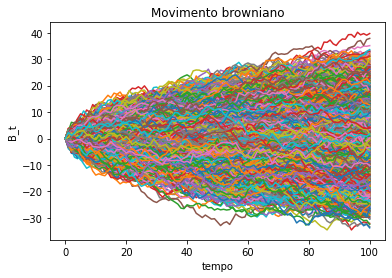
\includegraphics[width=1.0\linewidth]{bm.png}
 \caption{$10000$ caminhos movimentos browniano com $l=100$}
 \label{fig:bm}
\end{figure}
 
Uma vez que podemos simular o movimento browniano passamos  construir uma simulação da equação diferencial  estocástica \ref{crecimento} utilizando o seguinte esquema de Euler:
\[
x_{t_{n+1}}=x_{t_n}+rx_{t_n}(k-\alpha x_{t_n})(t_{n+1}-t_{n})+\beta x_{t_n}(B_{t_{n+1}}-B_{t_n})
\]
No nosso trabalho vamos simular a equação utilizando o esquema de Euler com a simulação do movimento browniano feita acima. É possível ver que o esquema de Euler fornece uma boa aproximação para estudar quantidades que dependem da lei do processo $x_t$ que é solução da equação a ser simulada. A aproximação é melhor quanto maior é a  discretização do tempo. No nosso caso discretizamos o tempo em intervalos de comprimento 1. No entanto, podem ser feitas discretizações mais precisas diminuindo o comprimento deste intervalo. O resultado que garante esta última afirmação é o teorema de Turelli que está apresentado em Gard(1988, p. 166,167). Descrevemos a seguir as ideias básicas deste resultado. 

Considere uma equação diferencial estocástica da forma 
\[dx_t = X_0(x_t)dt + X_1(x_t)dB_t\] em que  $X_0$ e $X_1$ são contínuas, diferenciáveis em $[0, \infty)$ e que satisfazem
\begin{itemize}
\item $X_0(0) = X_1(0) = 0.$
\item existe $R>0$ tal que se $x>R$ então $X_0(x)<0$
\item se $x\neq 0$ então $X_1(x)\neq 0$
\end{itemize} 
Assuma que para qualquer solução em $[0, \infty)$ o limite no $\infty$ é inatingivel, isto é 
\[
\mathbb{P}\left[\lim_{t\rightarrow\infty}x_t=\infty\right]=0
\] 
Seja $ \eta_M $ é uma sequencia de variáveis aleatórias com distribuição idéntica e independente, de média $0$, variância $1$ e terceiro momento finito ($E[\eta_M^3(i)] < \infty$ para todo $i$.)

Com isto, definimos  $x^M$  por :
\begin{eqnarray*}
x^M_{a+n+1}&=& x^M_{a+n} +  X_0^M(x^M_{a+n})\frac{1}{M} + X_1^M(x^M_{a+n})\frac{\eta_M(a+n+1)}{M^{\frac{1}{2}}}\\
x^M(a)&=& x_a
\end{eqnarray*}
e estendemos a um  processo estocástico  de tempo contínuo dado por:
\[
x^M(t) = x^M(a+n),\quad  a+n \leq t<a+n+1
\]
Com esta estrutura temos o seguinte resultado (GARD, 1988, p. 166, 167).
\begin{teo}[Turelli]
Com as hipóteses acima, se $x_t$ é solução da equação 
\[dx_t = X_0(x_t)dt + X_1(x_t)dB_t\] então 
\[
\lim_{M\rightarrow\infty}\mathbb{P}\left[|x^M(t)-x(t)|>\epsilon\right]=0.
\]

\end{teo}
 
Vamos mostrar agora que o esquema de Euler proposto acima para nossa equação satisfaz as condições do teorema de Turelli. Repetimos que aqui só vamos considerar o primeiro paso (que corresponde para $M=1$ e para partições no tempo em intervalos de comprimento 1), porém se aumentando o valor de $M$ teremos aproximações mais precisas. 

Assim, na equação do modelo de crescimento populacional que estamos considerando temos  que
\begin{itemize}
\item As funções 
\[X_0(x)= rx (k-\alpha x ),\quad X_1(x) = \beta x,\quad   x_0 = N,\]  satisfazem as hipóteses do teorema. 
\item O valor de $M$ está associado a partição do intervalo. No nosso caso, como dito acima, vamos somente trabalhar com $M=1$ e $\eta_1=(S_j)$ como na simulação do movimento browniano acima. Porém, no caso genérico teríamos que, para cada $M$, $\eta_M=(S_j)$ é uma sequência de variáveis aleatorias independentes com distribuição normal com media $0$ e variança $1$.  De fato,  como 
\[t_{i+1}-t_{i}=\frac{1}{M},\] temos que 
\[
\frac{\eta_M(i+1)}{\sqrt{M}}=\frac{1}{\sqrt{M}}S_{i+1}=\sqrt{t_{i+1}-t_i}S_{i+1}=(B_{t_{i+1}}-B_{t_i}).
\]
Decorre disto que o terceiro momento  da $\eta_M(i)$ é finito para cada $i$.
 \end{itemize} 
Agora, para poder utilizar o teorema de Turelli, só resta mostrar que o limite no $\infty$ é inatingível. Para isto vemos que a solução do processo satisfaz
\[
x_t=\frac{e^{\left(rk-\frac{1}{2}\beta^2\right)t+\beta B_t}}{\frac{1}{N}+r\alpha\int_0^te^{\left(rk-\frac{1}{2}\beta^2\right)s+\beta B_s}~ds}\leq Ne^{\left(rk-\frac{1}{2}\beta^2\right)t+\beta B_t}.
\]
agora, utilizando que $x_t>0$ e a desigualdade de Chebyshev(OKSENDAL, 1997, p. 16), temos que 
\begin{eqnarray*}
\mathbb{P}[x_t>\alpha]&\leq&\frac{1}{\alpha}\mathbb{E}[x_t]\\
&\leq&\frac{1}{\alpha}\mathbb{E}\left[Ne^{\left(rk-\frac{1}{2}\beta^2\right)t+\beta B_t}\right]\\
&=&\frac{N}{\alpha}e^{rkt}.
\end{eqnarray*}
Aqui foi utilizado o seguinte resultado. 


\begin{lem}\label{M_t}
\[M_t=e^{\left(rk-\frac{1}{2}\beta^2\right)t+\beta B_t}\]
satisfaz $\me[M_t]=e^{rkt}$.
\end{lem}

\begin{proof}
Utilizamos a fórmula de Itô para 
\[
f(t,x)=e^{\left(rk-\frac{1}{2}\beta^2\right)t+\beta x},
\]
então 
\[
f(t,B_t)=1+rk\int_0^tf(s,B_s)~ds+\beta\int_0^tf(s,B_s)~dB_s.
\]
Utilizando que 
\[\me\left[\beta\int_0^tf(s,B_s)~dB_s\right]=0,\]
obtemos 
\[
\me[f(t,B_t)]=1+rk\int_0^t\me[f(s,B_s)]~ds.
\]
De onde segue que,
\[
\me[f(t,B_t)]=e^{rkt}.
\]
\end{proof}


Com isto, temos mostrado que, para todo $t>0$, vale 
\[
\mathbb{P}[x_t=\infty]=\lim_{\alpha\rightarrow \infty}\mathbb{P}[x_t>\alpha]=0.
\]
Portanto o limite no $\infty$ é inatingível. 


Assim sendo, todas as hipótesis do Teorema de Turelli são satisfeitas e ele pode ser aplicado. Então, a simulação   $x^M$ que está asociada ao esquema de Euler apresentado, converge em lei à $x_t$ se $M \rightarrow \infty$. 


Aqui só vamos simular o caso em que $M=1$ pois para valores maiores de $M$ o tempo computacional é muito maior. A seguir, mostramos na figura \ref{fig:xt} uma simulação da solução $x_t$ com os seguintes parámetros
\[N=700 ,\quad r=0.0002 ,\quad\alpha=1 , \quad k=1000 \quad\textrm{e}\quad\beta=0.01 .\] Por se tratar de uma função exponencial, foi utilizado escala logarítmica no eixo y para melhor visualização do processo.

\begin{figure}[H]
 \centering
 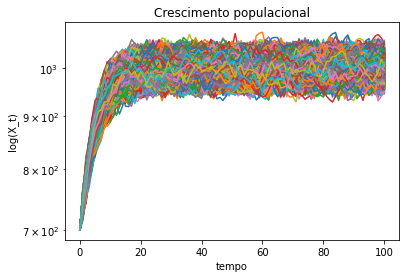
\includegraphics[width=1.0\linewidth]{xt.png}
 \caption{$10000$ caminhos $x^1$ com $l=100$}
 \label{fig:xt}
\end{figure}



Finalizamos o trabalho mostrando a consistência da simulação com a teoria vista na seção anterior. De fato, após simular os caminhos,  foi observada a distribuição de $x^1$ em $t={99}$. Este valor de $t$ se corresponte com a centésima marca do tempo e consideramos um  valor de tempo suficientemente grande já que $t=\infty$ não é possível de ser simulado. Comparamos assim a distribuição de probabilidade obtida dentre os $10.000$ caminhos no tempo $t_{99}$ e a distribuição dada pela medida invariante $\rho(x)$ obtida na secção anterior. Como apresentado abaixo na figura 3, é possível observar que a distruibuição simulada é muito semelhante à distribuição teórica $\rho(x)$. Na figura, o intervalo $[920,1080]$ é particionado em $100$ partes iguais e é computada a frequência normalizada em que $x^1$ atinge cada um destes subintervalos para o valor de $t_{99}$. Isto gera a distribuição em azul.
 
\begin{figure}[H]
 \centering
 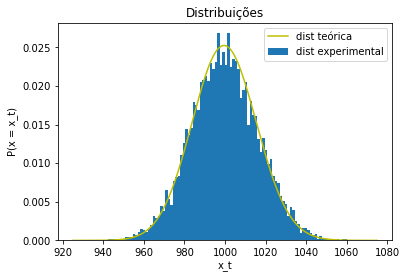
\includegraphics[width=1.0\linewidth]{dist.png}
 \caption{distribuição discreta de probabilidade em $t_{99}$ e distribuição da densidade da medida invariante $\rho(x)$}
 \label{fig:dist}
\end{figure}



 
\section{Apêndices} 

Neste apêndice apresentamos o código construído em python para as simulações, além do código, é disponibilizado através do github, um notebook criado originalmente no google colab onde é possível se ver a execução passo a passo e variar parâmetros para se observar os resultados obtidos. Fazendo testes experimentais com o intuito de melhor estimar os parâmetros para uma simulação apresentável, foi possível se observar que é interessante para a simulação que $rk < 1$, que $\beta$ seja da ordem de $\frac{\alpha rk}{10}$ para $\alpha > 0$ e da ordem de $rk$ para $\alpha = 0$ pois para valores fora dessa faixa o ruido é predominante na simulação e se faz necessário utilizar um número maior de simulações do movimento browniano (isto é, um valor $>10.000$) o que torna o tempo computacional muito maior.


\subsection*{Código em python}

\begin{lstlisting}[language=Python]
import numpy
import math
from matplotlib import pyplot as plt
from scipy.stats import gamma
import numpy as np

#calculo de x_t
def x_t2(r, K, alpha, beta, x_0, lista):
    out = [(lista[0][0],x_0)]
    outQuad = [(lista[0][0],x_0**2)]
    tamanho = len(lista)
    for i in range(1,tamanho):
      out.append((lista[i][0],out[i-1][1] + r*out[i-1][1]
      		*(K-alpha*out[i-1][1])
      		*(lista[i][0]-lista[i-1][0])+
      		beta*out[i-1][1]*(lista[i][1]-lista[i-1][1])))
      outQuad.append((lista[i][0],out[i][1]**2))

    return out, outQuad
    
#calculo esperanca dos caminhos simulados
def espSim(lista, pos):
    aux=0
    for i in range(len(lista)):
        aux+=lista[i][pos][1]
    return aux/len(lista)



alpha = 1
# parametros da simulacao 
n = 10000
k = 100
dt=1
t = [i*dt for i in range(k+1)]

if alpha != 0:
    r=0.0002
    K=1000 
    beta=0.01
    x_0=700
elif alpha == 0:
    r=0.0002
    K=1000 
    alpha=0
    beta=0.2
    x_0=2

B = [[0] for i in range(n)] #array com variaveis aleatorias 
S = [[] for i in range(n)] #array com as variaveis aleatorias S~N(0,1)

#simulacao  movimentos brownianos
for j in range(n):
    for i in range(k):
        S[j].append(numpy.random.normal(0,1))

for j in range(n):
    for i in range(k):
        B[j].append(B[j][i] + dt**0.5*S[j][i])

#criacao de tuplas(tempo, movimento browniano)
lista = [[] for i in range(n)]
for j in range(n):
    for i in range(k+1):
        lista[j].append((t[i], B[j][i]))

plt.title('Movimento browniano')
plt.xlabel('tempo')
plt.ylabel('B_t')

for i in range(n):
  plt.plot(*zip(*lista[i]))

plt.title('Movimento browniano')
plt.xlabel('tempo')
plt.ylabel('B_t')



#calculo da variavel aleatoria x_t
lista2 = [[] for i in range(n)]
lista3 = [[] for i in range(n)]
for j in range(n):
    x, x2 = x_t2(r,K,alpha,beta,x_0, lista[j])
    lista2[j] = x
    lista3[j] = x2


for i in range(n):
    plt.semilogy(*zip(*lista2[i]), zorder = 1)
    
#calculo esperanca simulada
espSimul = []
for i in range(k+1):
    espSimul.append((t[i], espSim(lista2, i)))

espQuadSimul = []
for i in range(k+1):
    espQuadSimul.append((t[i], espSim(lista3, i)) )

sdevUp = [(t[i], espSimul[i][1]+(espQuadSimul[i][1] -
				 espSimul[i][1]**2)**0.5)
				 for i in range(len(espQuadSimul))]
sdevDown = [(t[i], espSimul[i][1]-(espQuadSimul[i][1] -
				 espSimul[i][1]**2)**0.5)
				 for i in range(len(espQuadSimul))]

#plot caminhos e esperancas
plt.title('Crescimento populacional, alfa='+str(alpha))
plt.xlabel('tempo')
plt.ylabel('log(X_t)')

plt.semilogy(*zip(*espSimul), linewidth=3, color='brown', zorder=2)
plt.semilogy(*zip(*sdevUp), linewidth=3, color='blue', zorder =2)
plt.semilogy(*zip(*sdevDown), linewidth=3, color='blue', zorder =2)

for i in range(n):
    plt.semilogy(*zip(*lista2[i]), zorder = 1)

legenda = []
legenda.append("Esperanca simulada")
legenda.append("Desvio padrao")


plt.legend(legenda)


if alpha != 0:
  a, c = (2*r*K-beta**2)/(beta**2), 2*r*alpha/beta**2
  aux = [lista2[i][k][1] for i in range(len(lista2))]

  fig, ax = plt.subplots(1, 1)

  x = np.linspace (925, 1075, 4000) 
  y1 = gamma.pdf(x, a=a, scale=1/c)
  ax.plot(x, y1, "y-", label=(r'$\alpha=29, \beta=3$')) 

  ax.hist(aux, 100, density=True)

  ax.set_title('Distribuicoes')
  ax.set_xlabel('x_t')
  ax.set_ylabel('P(x = x_t)')

  legenda2 = []
  legenda2.append('dist teorica')
  legenda2.append('dist experimental')

  ax.legend(legenda2)


  print((2*r*K-beta**2)/(2*r*alpha))


\end{lstlisting}
O código está também disponível no github em:

\href{URL}{https://github.com/HitaloCesar/artigo-cres-pop/blob/main/simul.ipynb}

\section{Agradecimentos}
Hitalo Cesar Alves agradece ao CNPq pelo suporte dado via a bolsa PICME para seus estudos de iniciação científica.

\noindent Diego Sebastian Ledesma recebeu suporte financeiro da Coordenação de Aperfeiçoamento de
Pessoal de Nível Superior - Brasil (CAPES) - Finance Code 001 e Fapesp 
2020/04426-6 e 2018/13481-0.  


\Referenciasbibliograficas


\begin{flushleft}

GARD, T. C. \textbf{Introduction to stochastic differential equations}. New York: Marcel Dekker Inc, 1988.

\

KHASMINSKII, R. \textbf{Stochastic stability of differential equations}. [cidade]: Springer, 2011.(Stochastic modelling and applied probability book series).

\

KUNITA, H. \textbf{Stochastic flows and stochastic differential equations}. Cambridge: Cambridge University Press, 1997.	

\

OKSENDAL, B. \textbf{Stochastic differential equations:} an introduction with applications. Berlin, Heidelberg: Springer-Verlag, 1997.
	
\	
	
POLANSKY, P.  Invariant distributions for multipopulation models in
random environments,  \textbf{Theor. Pop. Biol.}, v. 16, n. 1, p. 25-34, 1979.	

\

SONDERMAN, D. \textbf{Introduction to stochastic calculus for finance.} Berlin, Heidelberg: Springer-Verlag, 2006. (Lecture Notes in Economics and Mathematical Systems, 579).
\	
	
	
	
	
\end{flushleft}


\end{document}